\section{点、直线和平面}

本节介绍两个三维空间中最基础的几何体——点、直线和平面。

本节要点:
\begin{itemize}
    \item 掌握点、直线和平面的矢量表达式。
\end{itemize}

%============================================================
\subsection{点}

\begin{definition}[点]
三维空间的点用三个坐标值描述,通常写为$\mathrm{P}\left( x,y,z \right) $,也可缩写为“点$\mathrm{P}$”,也可以用矢量表示为“点$\boldsymbol{p}=\left( x\,\,y\,\,z \right) ^T$”。
\end{definition}

为符合矢量的加法运算法则,规定过两点$\mathrm{P}_1\left( x_1,y_1,z_1 \right) ,\mathrm{P}_2\left( x_2,y_2,z_2 \right) $且方向从$\mathrm{P}_1$到$\mathrm{P}_2$的直线,写成:
\begin{align*}
\overrightarrow{\mathrm{P}_1\mathrm{P}_2}:&=\boldsymbol{p}_2-\boldsymbol{p}_1 \\
&=\left( x_2\,\,y_2\,\,z_2 \right) ^T-\left( x_1\,\,y_1\,\,z_1 \right) ^T \\
&=\left( x_2-x_1 \quad y_2-y_1 \quad z_2-z_1 \right) ^T
\end{align*}
如果方向从$\mathrm{P}_2$到$\mathrm{P}_1$,则有$\overrightarrow{\mathrm{P}_2\mathrm{P}_1}=\boldsymbol{p}_1-\boldsymbol{p}_2=-\overrightarrow{\mathrm{P}_1\mathrm{P}_2}$。

\begin{figure}[h]
\centering
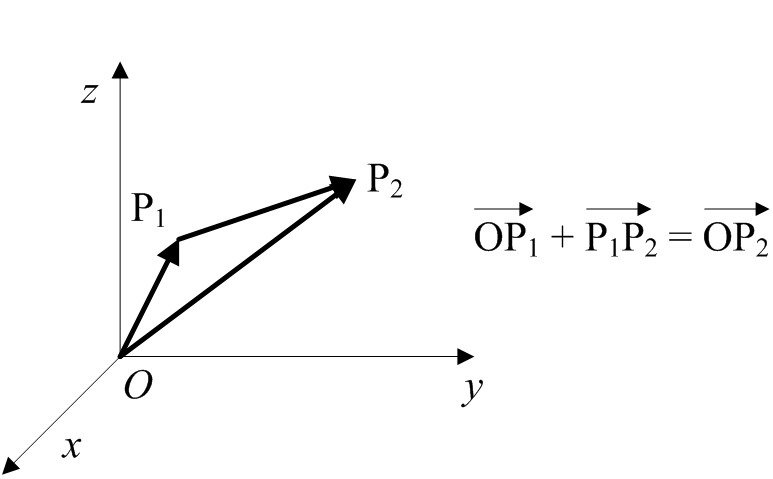
\includegraphics[height=4cm]{5.1.png}
\end{figure}

%============================================================
\subsection{直线方程}

\begin{definition}[直线方程]
若空间中两点$\boldsymbol{p},\boldsymbol{p}_0$构成的直线$\boldsymbol{p}-\boldsymbol{p}_0$和方向$\boldsymbol{n}=\left( A\,\,B\,\,C \right) ^T$平行,这些点构成的几何体称为{\bf 直线},用矢量方程描述为:
\[
\boldsymbol{p}-\boldsymbol{p}_0=\lambda \boldsymbol{n}
\]
展开后:
\[
\left( \begin{array}{c}
	x\\
	y\\
	z\\
\end{array} \right) -\left( \begin{array}{c}
	x_0\\
	y_0\\
	z_0\\
\end{array} \right) =\lambda \left( \begin{array}{c}
	A\\
	B\\
	C\\
\end{array} \right) \quad \text{或} \quad \frac{x-x_0}{A}=\frac{y-y_0}{B}=\frac{z-z_0}{C}
\]
称为{\bf 直线方程},其中:
\begin{itemize}
    \item $\boldsymbol{n}=\left( A\,\,B\,\,C \right) ^T$:直线的方向;
    \item $\boldsymbol{p}_0=\left( x_0\,\,y_0\,\,z_0 \right) ^T$:已知的直线上的点。
\end{itemize}
\end{definition}

若两直线平行,则两个矢量方向可以一致也可以相反。
如无特别情况,我们取一致的方向。

直线的另一种表达方式是两个平面的交线,若有两个平面:
\[
\begin{cases}
	A_1x+B_1y+C_1z+D_1=0\\
	A_2x+B_2y+C_2z+D_2=0\\
\end{cases}
\]
转化成点向式方程的步骤:
\begin{enumerate}
    \item 找出直线上的点$\boldsymbol{p}_0=\left( x_0\,\,y_0\,\,z_0 \right) ^T$,通常方便起见取$z_0=0$计算。
    \item 找出方向,直线的方向$\boldsymbol{n}=\left( A\,\,B\,\,C \right) ^T$和两个平面的法向构成的平面垂直,即:
    \[
    \boldsymbol{n}=\boldsymbol{n}_1\times \boldsymbol{n}_2=\left| \begin{matrix}
        \mathbf{i}&		\mathbf{j}&		\mathbf{k}\\
        A_1&		B_1&		C_1\\
        A_2&		B_2&		C_2\\
    \end{matrix} \right|
    \]
\end{enumerate}

%============================================================
\subsection{平面方程}

\begin{definition}[平面方程]
若点$\boldsymbol{p},\boldsymbol{p}_0$构成的直线$\boldsymbol{p}-\boldsymbol{p}_0$和方向$\boldsymbol{n}=\left( A\,\,B\,\,C \right) ^T$(称为{\bf 该平面的法向方向})垂直,这些点构成的几何体称为{\bf 平面},用矢量方程描述为:
\[
\left( \boldsymbol{p}-\boldsymbol{p}_0 \right) ^T\boldsymbol{n}=0
\]
展开后:
\begin{align*}
A\left( x-x_0 \right) +B\left( y-y_0 \right) +C\left( z-z_0 \right) =0 \quad \text{或} \quad Ax+By+Cz+D=0
\end{align*}
称为{\bf 平面方程},其中:
\begin{itemize}
    \item $\boldsymbol{p}-\boldsymbol{p}_0$:平面的法向;
    \item $\boldsymbol{p}_0=\left( x_0\,\,y_0\,\,z_0 \right) ^T$:已知的平面上的点。
\end{itemize}
\end{definition}

特别地,当平面和{\it xyz}三轴分别交于$x_0,y_0,z_0$,则可以写成截距式:
\[
\frac{x}{x_0}+\frac{y}{y_0}+\frac{z}{z_0}=1
\]

%============================================================
\subsection{曲线方程和曲面方程}

\begin{definition}[曲面方程]
三维空间中的曲面都可以描述为关于点$\boldsymbol{p}$的隐函数,如:
\[
F\left( \boldsymbol{p} \right) =0 \quad \text{或} \quad F\left( x,y,z \right) =0 \quad \text{或} \quad z=z\left( x,y \right)
\]
称为{\bf 曲面方程}。
\end{definition}

\begin{definition}[曲线方程]
在曲面方程中,$z$和$x,y$有约束关系,$x,y$之间并没有约束关系。
如果$x,y$之间还有约束关系,则曲面退化为曲线,上述表达式变为:
\[
F\left( x,y\left( x \right) ,z\left(y\left( x \right) \right) \right) =0 \quad \text{或} \quad z=z\left( x,y\left( x \right) \right)
\]
称为{\bf 曲线方程},更一般地,我们写成:
\[
\left\{ \begin{array}{c}
	x=x\left( t \right)\\
	y=y\left( t \right)\\
	z=z\left( t \right)\\
\end{array} \right.
\]
\end{definition}

\begin{tcolorbox}
这里并不刻意区分直线和平面的方向,直线的前后方向、平面的两侧方向,现在来讲都没有意义。
到了环流量和通量(即第二类曲线曲面积分),再规定线和面的方向。
\end{tcolorbox}




